\documentclass[1p]{elsarticle_modified}
%\bibliographystyle{elsarticle-num}

%\usepackage[colorlinks]{hyperref}
%\usepackage{abbrmath_seonhwa} %\Abb, \Ascr, \Acal ,\Abf, \Afrak
\usepackage{amsfonts}
\usepackage{amssymb}
\usepackage{amsmath}
\usepackage{amsthm}
\usepackage{scalefnt}
\usepackage{amsbsy}
\usepackage{kotex}
\usepackage{caption}
\usepackage{subfig}
\usepackage{color}
\usepackage{graphicx}
\usepackage{xcolor} %% white, black, red, green, blue, cyan, magenta, yellow
\usepackage{float}
\usepackage{setspace}
\usepackage{hyperref}

\usepackage{tikz}
\usetikzlibrary{arrows}

\usepackage{multirow}
\usepackage{array} % fixed length table
\usepackage{hhline}

%%%%%%%%%%%%%%%%%%%%%
\makeatletter
\renewcommand*\env@matrix[1][\arraystretch]{%
	\edef\arraystretch{#1}%
	\hskip -\arraycolsep
	\let\@ifnextchar\new@ifnextchar
	\array{*\c@MaxMatrixCols c}}
\makeatother %https://tex.stackexchange.com/questions/14071/how-can-i-increase-the-line-spacing-in-a-matrix
%%%%%%%%%%%%%%%

\usepackage[normalem]{ulem}

\newcommand{\msout}[1]{\ifmmode\text{\sout{\ensuremath{#1}}}\else\sout{#1}\fi}
%SOURCE: \msout is \stkout macro in https://tex.stackexchange.com/questions/20609/strikeout-in-math-mode

\newcommand{\cancel}[1]{
	\ifmmode
	{\color{red}\msout{#1}}
	\else
	{\color{red}\sout{#1}}
	\fi
}

\newcommand{\add}[1]{
	{\color{blue}\uwave{#1}}
}

\newcommand{\replace}[2]{
	\ifmmode
	{\color{red}\msout{#1}}{\color{blue}\uwave{#2}}
	\else
	{\color{red}\sout{#1}}{\color{blue}\uwave{#2}}
	\fi
}

\newcommand{\Sol}{\mathcal{S}} %segment
\newcommand{\D}{D} %diagram
\newcommand{\A}{\mathcal{A}} %arc


%%%%%%%%%%%%%%%%%%%%%%%%%%%%%5 test

\def\sl{\operatorname{\textup{SL}}(2,\Cbb)}
\def\psl{\operatorname{\textup{PSL}}(2,\Cbb)}
\def\quan{\mkern 1mu \triangleright \mkern 1mu}

\theoremstyle{definition}
\newtheorem{thm}{Theorem}[section]
\newtheorem{prop}[thm]{Proposition}
\newtheorem{lem}[thm]{Lemma}
\newtheorem{ques}[thm]{Question}
\newtheorem{cor}[thm]{Corollary}
\newtheorem{defn}[thm]{Definition}
\newtheorem{exam}[thm]{Example}
\newtheorem{rmk}[thm]{Remark}
\newtheorem{alg}[thm]{Algorithm}

\newcommand{\I}{\sqrt{-1}}
\begin{document}

%\begin{frontmatter}
%
%\title{Boundary parabolic representations of knots up to 8 crossings}
%
%%% Group authors per affiliation:
%\author{Yunhi Cho} 
%\address{Department of Mathematics, University of Seoul, Seoul, Korea}
%\ead{yhcho@uos.ac.kr}
%
%
%\author{Seonhwa Kim} %\fnref{s_kim}}
%\address{Center for Geometry and Physics, Institute for Basic Science, Pohang, 37673, Korea}
%\ead{ryeona17@ibs.re.kr}
%
%\author{Hyuk Kim}
%\address{Department of Mathematical Sciences, Seoul National University, Seoul 08826, Korea}
%\ead{hyukkim@snu.ac.kr}
%
%\author{Seokbeom Yoon}
%\address{Department of Mathematical Sciences, Seoul National University, Seoul, 08826,  Korea}
%\ead{sbyoon15@snu.ac.kr}
%
%\begin{abstract}
%We find all boundary parabolic representation of knots up to 8 crossings.
%
%\end{abstract}
%\begin{keyword}
%    \MSC[2010] 57M25 
%\end{keyword}
%
%\end{frontmatter}

%\linenumbers
%\tableofcontents
%
\newcommand\colored[1]{\textcolor{white}{\rule[-0.35ex]{0.8em}{1.4ex}}\kern-0.8em\color{red} #1}%
%\newcommand\colored[1]{\textcolor{white}{ #1}\kern-2.17ex	\textcolor{white}{ #1}\kern-1.81ex	\textcolor{white}{ #1}\kern-2.15ex\color{red}#1	}

{\Large $\underline{12n_{0863}~(K12n_{0863})}$}

\setlength{\tabcolsep}{10pt}
\renewcommand{\arraystretch}{1.6}
\vspace{1cm}\begin{tabular}{m{100pt}>{\centering\arraybackslash}m{274pt}}
\multirow{5}{120pt}{
	\centering
	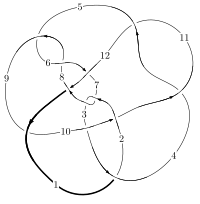
\includegraphics[width=112pt]{../../../GIT/diagram.site/Diagrams/png/2952_12n_0863.png}\\
\ \ \ A knot diagram\footnotemark}&
\allowdisplaybreaks
\textbf{Linearized knot diagam} \\
\cline{2-2}
 &
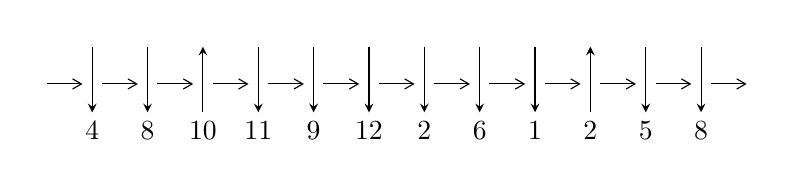
\begin{tikzpicture}[x=20pt, y=17pt]
	% nodes
	\node (C0) at (0, 0) {};
	\node (C1) at (1, 0) {};
	\node (C1U) at (1, +1) {};
	\node (C1D) at (1, -1) {4};

	\node (C2) at (2, 0) {};
	\node (C2U) at (2, +1) {};
	\node (C2D) at (2, -1) {8};

	\node (C3) at (3, 0) {};
	\node (C3U) at (3, +1) {};
	\node (C3D) at (3, -1) {10};

	\node (C4) at (4, 0) {};
	\node (C4U) at (4, +1) {};
	\node (C4D) at (4, -1) {11};

	\node (C5) at (5, 0) {};
	\node (C5U) at (5, +1) {};
	\node (C5D) at (5, -1) {9};

	\node (C6) at (6, 0) {};
	\node (C6U) at (6, +1) {};
	\node (C6D) at (6, -1) {12};

	\node (C7) at (7, 0) {};
	\node (C7U) at (7, +1) {};
	\node (C7D) at (7, -1) {2};

	\node (C8) at (8, 0) {};
	\node (C8U) at (8, +1) {};
	\node (C8D) at (8, -1) {6};

	\node (C9) at (9, 0) {};
	\node (C9U) at (9, +1) {};
	\node (C9D) at (9, -1) {1};

	\node (C10) at (10, 0) {};
	\node (C10U) at (10, +1) {};
	\node (C10D) at (10, -1) {2};

	\node (C11) at (11, 0) {};
	\node (C11U) at (11, +1) {};
	\node (C11D) at (11, -1) {5};

	\node (C12) at (12, 0) {};
	\node (C12U) at (12, +1) {};
	\node (C12D) at (12, -1) {8};
	\node (C13) at (13, 0) {};

	% arrows
	\draw[->,>={angle 60}]
	(C0) edge (C1) (C1) edge (C2) (C2) edge (C3) (C3) edge (C4) (C4) edge (C5) (C5) edge (C6) (C6) edge (C7) (C7) edge (C8) (C8) edge (C9) (C9) edge (C10) (C10) edge (C11) (C11) edge (C12) (C12) edge (C13) ;	\draw[->,>=stealth]
	(C1U) edge (C1D) (C2U) edge (C2D) (C3D) edge (C3U) (C4U) edge (C4D) (C5U) edge (C5D) (C6U) edge (C6D) (C7U) edge (C7D) (C8U) edge (C8D) (C9U) edge (C9D) (C10D) edge (C10U) (C11U) edge (C11D) (C12U) edge (C12D) ;
	\end{tikzpicture} \\
\hhline{~~} \\& 
\textbf{Solving Sequence} \\ \cline{2-2} 
 &
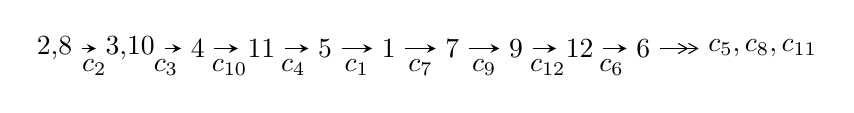
\begin{tikzpicture}[x=23pt, y=7pt]
	% node
	\node (A0) at (-1/8, 0) {2,8};
	\node (A1) at (17/16, 0) {3,10};
	\node (A2) at (17/8, 0) {4};
	\node (A3) at (25/8, 0) {11};
	\node (A4) at (33/8, 0) {5};
	\node (A5) at (41/8, 0) {1};
	\node (A6) at (49/8, 0) {7};
	\node (A7) at (57/8, 0) {9};
	\node (A8) at (65/8, 0) {12};
	\node (A9) at (73/8, 0) {6};
	\node (C1) at (1/2, -1) {$c_{2}$};
	\node (C2) at (13/8, -1) {$c_{3}$};
	\node (C3) at (21/8, -1) {$c_{10}$};
	\node (C4) at (29/8, -1) {$c_{4}$};
	\node (C5) at (37/8, -1) {$c_{1}$};
	\node (C6) at (45/8, -1) {$c_{7}$};
	\node (C7) at (53/8, -1) {$c_{9}$};
	\node (C8) at (61/8, -1) {$c_{12}$};
	\node (C9) at (69/8, -1) {$c_{6}$};
	\node (A10) at (11, 0) {$c_{5},c_{8},c_{11}$};

	% edge
	\draw[->,>=stealth]	
	(A0) edge (A1) (A1) edge (A2) (A2) edge (A3) (A3) edge (A4) (A4) edge (A5) (A5) edge (A6) (A6) edge (A7) (A7) edge (A8) (A8) edge (A9) ;
	\draw[->>,>={angle 60}]	
	(A9) edge (A10);
\end{tikzpicture} \\ 

\end{tabular} \\

\footnotetext{
The image of knot diagram is generated by the software ``\textbf{Draw programme}" developed by Andrew Bartholomew(\url{http://www.layer8.co.uk/maths/draw/index.htm\#Running-draw}), where we modified some parts for our purpose(\url{https://github.com/CATsTAILs/LinksPainter}).
}\phantom \\ \newline 
\centering \textbf{Ideals for irreducible components\footnotemark of $X_{\text{par}}$} 
 
\begin{align*}
I^u_{1}&=\langle 
1.48412\times10^{552} u^{104}+1.20399\times10^{552} u^{103}+\cdots+1.12741\times10^{553} b-4.63442\times10^{554},\\
\phantom{I^u_{1}}&\phantom{= \langle  }3.55029\times10^{554} u^{104}+2.93066\times10^{554} u^{103}+\cdots+6.42625\times10^{554} a-1.17419\times10^{557},\\
\phantom{I^u_{1}}&\phantom{= \langle  }u^{105}+u^{104}+\cdots-170 u-57\rangle \\
I^u_{2}&=\langle 
1.77671\times10^{24} u^{32}+1.53488\times10^{24} u^{31}+\cdots+1.44503\times10^{24} b-5.63759\times10^{24},\\
\phantom{I^u_{2}}&\phantom{= \langle  }8.36483\times10^{24} u^{32}+5.76140\times10^{24} u^{31}+\cdots+1.44503\times10^{24} a-2.52600\times10^{25},\;u^{33}+5 u^{31}+\cdots-2 u+1\rangle \\
\\
\end{align*}
\raggedright * 2 irreducible components of $\dim_{\mathbb{C}}=0$, with total 138 representations.\\
\footnotetext{All coefficients of polynomials are rational numbers. But the coefficients are sometimes approximated in decimal forms when there is not enough margin.}
\newpage
\renewcommand{\arraystretch}{1}
\centering \section*{I. $I^u_{1}= \langle 1.48\times10^{552} u^{104}+1.20\times10^{552} u^{103}+\cdots+1.13\times10^{553} b-4.63\times10^{554},\;3.55\times10^{554} u^{104}+2.93\times10^{554} u^{103}+\cdots+6.43\times10^{554} a-1.17\times10^{557},\;u^{105}+u^{104}+\cdots-170 u-57 \rangle$}
\flushleft \textbf{(i) Arc colorings}\\
\begin{tabular}{m{7pt} m{180pt} m{7pt} m{180pt} }
\flushright $a_{2}=$&$\begin{pmatrix}1\\0\end{pmatrix}$ \\
\flushright $a_{8}=$&$\begin{pmatrix}0\\u\end{pmatrix}$ \\
\flushright $a_{3}=$&$\begin{pmatrix}1\\u^2\end{pmatrix}$ \\
\flushright $a_{10}=$&$\begin{pmatrix}-0.552466 u^{104}-0.456045 u^{103}+\cdots-517.092 u+182.718\\-0.131639 u^{104}-0.106792 u^{103}+\cdots-106.123 u+41.1066\end{pmatrix}$ \\
\flushright $a_{4}=$&$\begin{pmatrix}0.561311 u^{104}+0.459171 u^{103}+\cdots+482.206 u-177.562\\-0.00726235 u^{104}-0.00463571 u^{103}+\cdots+7.36074 u+2.13346\end{pmatrix}$ \\
\flushright $a_{11}=$&$\begin{pmatrix}-0.684105 u^{104}-0.562837 u^{103}+\cdots-623.216 u+223.824\\-0.131639 u^{104}-0.106792 u^{103}+\cdots-106.123 u+41.1066\end{pmatrix}$ \\
\flushright $a_{5}=$&$\begin{pmatrix}-0.436986 u^{104}-0.362545 u^{103}+\cdots-426.067 u+147.107\\-0.204326 u^{104}-0.164531 u^{103}+\cdots-152.977 u+63.6197\end{pmatrix}$ \\
\flushright $a_{1}=$&$\begin{pmatrix}-0.0563406 u^{104}-0.0414995 u^{103}+\cdots-13.6473 u+14.1812\\0.199358 u^{104}+0.160284 u^{103}+\cdots+145.605 u-61.6449\end{pmatrix}$ \\
\flushright $a_{7}=$&$\begin{pmatrix}u\\u\end{pmatrix}$ \\
\flushright $a_{9}=$&$\begin{pmatrix}-0.642845 u^{104}-0.522829 u^{103}+\cdots-541.471 u+206.336\\0.232514 u^{104}+0.186815 u^{103}+\cdots+159.915 u-71.2101\end{pmatrix}$ \\
\flushright $a_{12}=$&$\begin{pmatrix}-0.0563406 u^{104}-0.0414995 u^{103}+\cdots-13.6473 u+14.1812\\0.202183 u^{104}+0.162480 u^{103}+\cdots+146.294 u-62.4908\end{pmatrix}$ \\
\flushright $a_{6}=$&$\begin{pmatrix}0.00569159 u^{104}+0.00768304 u^{103}+\cdots+48.7098 u-14.8581\\-0.0142608 u^{104}-0.0142884 u^{103}+\cdots-13.3992 u+6.38063\end{pmatrix}$\\&\end{tabular}
\flushleft \textbf{(ii) Obstruction class $= -1$}\\~\\
\flushleft \textbf{(iii) Cusp Shapes $= 0.0298050 u^{104}+0.0240412 u^{103}+\cdots-80.5730 u+3.74527$}\\~\\
\newpage\renewcommand{\arraystretch}{1}
\flushleft \textbf{(iv) u-Polynomials at the component}\newline \\
\begin{tabular}{m{50pt}|m{274pt}}
Crossings & \hspace{64pt}u-Polynomials at each crossing \\
\hline $$\begin{aligned}c_{1}\end{aligned}$$&$\begin{aligned}
&u^{105}-6 u^{104}+\cdots-1036 u-76
\end{aligned}$\\
\hline $$\begin{aligned}c_{2},c_{7}\end{aligned}$$&$\begin{aligned}
&u^{105}+u^{104}+\cdots-170 u-57
\end{aligned}$\\
\hline $$\begin{aligned}c_{3}\end{aligned}$$&$\begin{aligned}
&u^{105}-3 u^{104}+\cdots-79493 u+29383
\end{aligned}$\\
\hline $$\begin{aligned}c_{4},c_{11}\end{aligned}$$&$\begin{aligned}
&u^{105}-5 u^{104}+\cdots+1974185 u+408799
\end{aligned}$\\
\hline $$\begin{aligned}c_{5},c_{8}\end{aligned}$$&$\begin{aligned}
&u^{105}-4 u^{104}+\cdots-703 u+103
\end{aligned}$\\
\hline $$\begin{aligned}c_{6}\end{aligned}$$&$\begin{aligned}
&u^{105}+u^{104}+\cdots+52772864 u+12173312
\end{aligned}$\\
\hline $$\begin{aligned}c_{9}\end{aligned}$$&$\begin{aligned}
&u^{105}+4 u^{104}+\cdots-34152 u-90143
\end{aligned}$\\
\hline $$\begin{aligned}c_{10}\end{aligned}$$&$\begin{aligned}
&u^{105}+4 u^{103}+\cdots-15298 u-4321
\end{aligned}$\\
\hline $$\begin{aligned}c_{12}\end{aligned}$$&$\begin{aligned}
&u^{105}+15 u^{103}+\cdots-9777498 u-803449
\end{aligned}$\\
\hline
\end{tabular}\\~\\
\newpage\renewcommand{\arraystretch}{1}
\flushleft \textbf{(v) Riley Polynomials at the component}\newline \\
\begin{tabular}{m{50pt}|m{274pt}}
Crossings & \hspace{64pt}Riley Polynomials at each crossing \\
\hline $$\begin{aligned}c_{1}\end{aligned}$$&$\begin{aligned}
&y^{105}-38 y^{104}+\cdots+1131816 y-5776
\end{aligned}$\\
\hline $$\begin{aligned}c_{2},c_{7}\end{aligned}$$&$\begin{aligned}
&y^{105}+71 y^{104}+\cdots+115084 y-3249
\end{aligned}$\\
\hline $$\begin{aligned}c_{3}\end{aligned}$$&$\begin{aligned}
&y^{105}-25 y^{104}+\cdots+61420019161 y-863360689
\end{aligned}$\\
\hline $$\begin{aligned}c_{4},c_{11}\end{aligned}$$&$\begin{aligned}
&y^{105}-67 y^{104}+\cdots+5174846874963 y-167116622401
\end{aligned}$\\
\hline $$\begin{aligned}c_{5},c_{8}\end{aligned}$$&$\begin{aligned}
&y^{105}+58 y^{104}+\cdots+102603 y-10609
\end{aligned}$\\
\hline $$\begin{aligned}c_{6}\end{aligned}$$&$\begin{aligned}
&y^{105}+7 y^{104}+\cdots-4512411558084608 y-148189525049344
\end{aligned}$\\
\hline $$\begin{aligned}c_{9}\end{aligned}$$&$\begin{aligned}
&y^{105}+28 y^{104}+\cdots-370452665546 y-8125760449
\end{aligned}$\\
\hline $$\begin{aligned}c_{10}\end{aligned}$$&$\begin{aligned}
&y^{105}+8 y^{104}+\cdots+2003573366 y-18671041
\end{aligned}$\\
\hline $$\begin{aligned}c_{12}\end{aligned}$$&$\begin{aligned}
&y^{105}+30 y^{104}+\cdots-43751002199554 y-645530295601
\end{aligned}$\\
\hline
\end{tabular}\\~\\
\newpage\flushleft \textbf{(vi) Complex Volumes and Cusp Shapes}
$$\begin{array}{c|c|c}  
\text{Solutions to }I^u_{1}& \I (\text{vol} + \sqrt{-1}CS) & \text{Cusp shape}\\
 \hline 
\begin{aligned}
u &= \phantom{-}1.00885\phantom{ +0.000000I} \\
a &= -1.06197\phantom{ +0.000000I} \\
b &= -0.898102\phantom{ +0.000000I}\end{aligned}
 & -5.78725\phantom{ +0.000000I} & \phantom{-0.000000 } 0 \\ \hline\begin{aligned}
u &= \phantom{-}0.348195 + 0.965456 I \\
a &= -0.662421 - 1.025780 I \\
b &= \phantom{-}0.710406 - 0.058573 I\end{aligned}
 & \phantom{-}2.72409 - 1.77279 I & \phantom{-0.000000 } 0 \\ \hline\begin{aligned}
u &= \phantom{-}0.348195 - 0.965456 I \\
a &= -0.662421 + 1.025780 I \\
b &= \phantom{-}0.710406 + 0.058573 I\end{aligned}
 & \phantom{-}2.72409 + 1.77279 I & \phantom{-0.000000 } 0 \\ \hline\begin{aligned}
u &= -0.882405 + 0.553989 I \\
a &= -0.074437 - 1.234280 I \\
b &= -0.803484 - 0.350969 I\end{aligned}
 & -3.02144 + 4.95106 I & \phantom{-0.000000 } 0 \\ \hline\begin{aligned}
u &= -0.882405 - 0.553989 I \\
a &= -0.074437 + 1.234280 I \\
b &= -0.803484 + 0.350969 I\end{aligned}
 & -3.02144 - 4.95106 I & \phantom{-0.000000 } 0 \\ \hline\begin{aligned}
u &= -1.048450 + 0.016990 I \\
a &= \phantom{-}0.150121 + 0.243755 I \\
b &= \phantom{-}0.887919 + 0.754009 I\end{aligned}
 & \phantom{-}2.85999 + 1.67647 I & \phantom{-0.000000 } 0 \\ \hline\begin{aligned}
u &= -1.048450 - 0.016990 I \\
a &= \phantom{-}0.150121 - 0.243755 I \\
b &= \phantom{-}0.887919 - 0.754009 I\end{aligned}
 & \phantom{-}2.85999 - 1.67647 I & \phantom{-0.000000 } 0 \\ \hline\begin{aligned}
u &= -0.039793 + 0.949685 I \\
a &= -0.94004 + 2.15880 I \\
b &= \phantom{-}0.325952 + 0.295385 I\end{aligned}
 & \phantom{-}1.139280 + 0.028861 I & \phantom{-0.000000 } 0 \\ \hline\begin{aligned}
u &= -0.039793 - 0.949685 I \\
a &= -0.94004 - 2.15880 I \\
b &= \phantom{-}0.325952 - 0.295385 I\end{aligned}
 & \phantom{-}1.139280 - 0.028861 I & \phantom{-0.000000 } 0 \\ \hline\begin{aligned}
u &= \phantom{-}0.154833 + 1.061630 I \\
a &= -0.189881 - 0.985439 I \\
b &= \phantom{-}0.219686 - 0.887030 I\end{aligned}
 & \phantom{-}3.52843 + 0.34309 I & \phantom{-0.000000 } 0\\
 \hline 
 \end{array}$$\newpage$$\begin{array}{c|c|c}  
\text{Solutions to }I^u_{1}& \I (\text{vol} + \sqrt{-1}CS) & \text{Cusp shape}\\
 \hline 
\begin{aligned}
u &= \phantom{-}0.154833 - 1.061630 I \\
a &= -0.189881 + 0.985439 I \\
b &= \phantom{-}0.219686 + 0.887030 I\end{aligned}
 & \phantom{-}3.52843 - 0.34309 I & \phantom{-0.000000 } 0 \\ \hline\begin{aligned}
u &= -0.103126 + 1.071570 I \\
a &= \phantom{-}2.55043 - 0.88486 I \\
b &= -0.460766 - 0.226733 I\end{aligned}
 & \phantom{-}1.67730 - 0.43540 I & \phantom{-0.000000 } 0 \\ \hline\begin{aligned}
u &= -0.103126 - 1.071570 I \\
a &= \phantom{-}2.55043 + 0.88486 I \\
b &= -0.460766 + 0.226733 I\end{aligned}
 & \phantom{-}1.67730 + 0.43540 I & \phantom{-0.000000 } 0 \\ \hline\begin{aligned}
u &= \phantom{-}0.280394 + 1.046660 I \\
a &= -0.855336 - 0.998668 I \\
b &= \phantom{-}0.279498 + 0.422370 I\end{aligned}
 & \phantom{-}3.38541 + 4.37298 I & \phantom{-0.000000 } 0 \\ \hline\begin{aligned}
u &= \phantom{-}0.280394 - 1.046660 I \\
a &= -0.855336 + 0.998668 I \\
b &= \phantom{-}0.279498 - 0.422370 I\end{aligned}
 & \phantom{-}3.38541 - 4.37298 I & \phantom{-0.000000 } 0 \\ \hline\begin{aligned}
u &= \phantom{-}0.865149 + 0.289940 I \\
a &= \phantom{-}0.448533 - 0.229635 I \\
b &= -0.572847 + 0.285068 I\end{aligned}
 & \phantom{-}3.17390 + 3.61321 I & \phantom{-0.000000 } 0 \\ \hline\begin{aligned}
u &= \phantom{-}0.865149 - 0.289940 I \\
a &= \phantom{-}0.448533 + 0.229635 I \\
b &= -0.572847 - 0.285068 I\end{aligned}
 & \phantom{-}3.17390 - 3.61321 I & \phantom{-0.000000 } 0 \\ \hline\begin{aligned}
u &= -0.192554 + 1.080830 I \\
a &= -1.13241 + 0.91785 I \\
b &= \phantom{-}0.369316 - 0.142754 I\end{aligned}
 & \phantom{-}0.364601 - 1.008040 I & \phantom{-0.000000 } 0 \\ \hline\begin{aligned}
u &= -0.192554 - 1.080830 I \\
a &= -1.13241 - 0.91785 I \\
b &= \phantom{-}0.369316 + 0.142754 I\end{aligned}
 & \phantom{-}0.364601 + 1.008040 I & \phantom{-0.000000 } 0 \\ \hline\begin{aligned}
u &= -1.106130 + 0.022263 I \\
a &= \phantom{-}0.304230 + 0.064905 I \\
b &= -0.620472 - 0.284639 I\end{aligned}
 & -0.842858 + 0.577647 I & \phantom{-0.000000 } 0\\
 \hline 
 \end{array}$$\newpage$$\begin{array}{c|c|c}  
\text{Solutions to }I^u_{1}& \I (\text{vol} + \sqrt{-1}CS) & \text{Cusp shape}\\
 \hline 
\begin{aligned}
u &= -1.106130 - 0.022263 I \\
a &= \phantom{-}0.304230 - 0.064905 I \\
b &= -0.620472 + 0.284639 I\end{aligned}
 & -0.842858 - 0.577647 I & \phantom{-0.000000 } 0 \\ \hline\begin{aligned}
u &= -0.147308 + 1.132450 I \\
a &= \phantom{-}0.680847 + 0.558761 I \\
b &= -0.08074 - 1.91420 I\end{aligned}
 & \phantom{-}4.01128 - 4.49825 I & \phantom{-0.000000 } 0 \\ \hline\begin{aligned}
u &= -0.147308 - 1.132450 I \\
a &= \phantom{-}0.680847 - 0.558761 I \\
b &= -0.08074 + 1.91420 I\end{aligned}
 & \phantom{-}4.01128 + 4.49825 I & \phantom{-0.000000 } 0 \\ \hline\begin{aligned}
u &= -0.083055 + 1.237500 I \\
a &= -1.164870 + 0.253601 I \\
b &= \phantom{-}0.174375 - 0.050687 I\end{aligned}
 & -0.66575 - 1.62690 I & \phantom{-0.000000 } 0 \\ \hline\begin{aligned}
u &= -0.083055 - 1.237500 I \\
a &= -1.164870 - 0.253601 I \\
b &= \phantom{-}0.174375 + 0.050687 I\end{aligned}
 & -0.66575 + 1.62690 I & \phantom{-0.000000 } 0 \\ \hline\begin{aligned}
u &= \phantom{-}1.236050 + 0.239157 I \\
a &= \phantom{-}0.227848 - 0.167445 I \\
b &= -0.572645 + 0.208358 I\end{aligned}
 & \phantom{-}2.51261 - 5.54800 I & \phantom{-0.000000 } 0 \\ \hline\begin{aligned}
u &= \phantom{-}1.236050 - 0.239157 I \\
a &= \phantom{-}0.227848 + 0.167445 I \\
b &= -0.572645 - 0.208358 I\end{aligned}
 & \phantom{-}2.51261 + 5.54800 I & \phantom{-0.000000 } 0 \\ \hline\begin{aligned}
u &= \phantom{-}1.226200 + 0.357895 I \\
a &= -0.53776 - 1.86174 I \\
b &= \phantom{-}0.72445 - 1.71790 I\end{aligned}
 & -5.08876 - 5.11598 I & \phantom{-0.000000 } 0 \\ \hline\begin{aligned}
u &= \phantom{-}1.226200 - 0.357895 I \\
a &= -0.53776 + 1.86174 I \\
b &= \phantom{-}0.72445 + 1.71790 I\end{aligned}
 & -5.08876 + 5.11598 I & \phantom{-0.000000 } 0 \\ \hline\begin{aligned}
u &= \phantom{-}0.063832 + 1.295060 I \\
a &= \phantom{-}1.65525 - 0.34732 I \\
b &= -2.26657 + 0.80603 I\end{aligned}
 & -0.57254 - 2.89314 I & \phantom{-0.000000 } 0\\
 \hline 
 \end{array}$$\newpage$$\begin{array}{c|c|c}  
\text{Solutions to }I^u_{1}& \I (\text{vol} + \sqrt{-1}CS) & \text{Cusp shape}\\
 \hline 
\begin{aligned}
u &= \phantom{-}0.063832 - 1.295060 I \\
a &= \phantom{-}1.65525 + 0.34732 I \\
b &= -2.26657 - 0.80603 I\end{aligned}
 & -0.57254 + 2.89314 I & \phantom{-0.000000 } 0 \\ \hline\begin{aligned}
u &= -1.238160 + 0.463453 I \\
a &= \phantom{-}0.79304 - 1.45662 I \\
b &= \phantom{-}0.03881 - 1.52223 I\end{aligned}
 & -4.93497 + 2.84907 I & \phantom{-0.000000 } 0 \\ \hline\begin{aligned}
u &= -1.238160 - 0.463453 I \\
a &= \phantom{-}0.79304 + 1.45662 I \\
b &= \phantom{-}0.03881 + 1.52223 I\end{aligned}
 & -4.93497 - 2.84907 I & \phantom{-0.000000 } 0 \\ \hline\begin{aligned}
u &= -0.399911 + 1.275490 I \\
a &= -0.172192 + 0.478716 I \\
b &= \phantom{-}0.058675 + 1.256580 I\end{aligned}
 & -1.54838 + 3.08573 I & \phantom{-0.000000 } 0 \\ \hline\begin{aligned}
u &= -0.399911 - 1.275490 I \\
a &= -0.172192 - 0.478716 I \\
b &= \phantom{-}0.058675 - 1.256580 I\end{aligned}
 & -1.54838 - 3.08573 I & \phantom{-0.000000 } 0 \\ \hline\begin{aligned}
u &= \phantom{-}0.229126 + 1.346680 I \\
a &= -0.376831 - 0.495639 I \\
b &= \phantom{-}0.296690 - 1.284650 I\end{aligned}
 & \phantom{-}1.23760 - 8.74933 I & \phantom{-0.000000 } 0 \\ \hline\begin{aligned}
u &= \phantom{-}0.229126 - 1.346680 I \\
a &= -0.376831 + 0.495639 I \\
b &= \phantom{-}0.296690 + 1.284650 I\end{aligned}
 & \phantom{-}1.23760 + 8.74933 I & \phantom{-0.000000 } 0 \\ \hline\begin{aligned}
u &= -0.041520 + 1.372500 I \\
a &= \phantom{-}1.164370 + 0.676393 I \\
b &= -1.24873 - 1.66615 I\end{aligned}
 & \phantom{-}4.91419 + 6.34054 I & \phantom{-0.000000 } 0 \\ \hline\begin{aligned}
u &= -0.041520 - 1.372500 I \\
a &= \phantom{-}1.164370 - 0.676393 I \\
b &= -1.24873 + 1.66615 I\end{aligned}
 & \phantom{-}4.91419 - 6.34054 I & \phantom{-0.000000 } 0 \\ \hline\begin{aligned}
u &= \phantom{-}0.228098 + 1.362980 I \\
a &= \phantom{-}1.294570 - 0.291387 I \\
b &= -1.35669 + 0.81998 I\end{aligned}
 & -1.00864 - 4.56909 I & \phantom{-0.000000 } 0\\
 \hline 
 \end{array}$$\newpage$$\begin{array}{c|c|c}  
\text{Solutions to }I^u_{1}& \I (\text{vol} + \sqrt{-1}CS) & \text{Cusp shape}\\
 \hline 
\begin{aligned}
u &= \phantom{-}0.228098 - 1.362980 I \\
a &= \phantom{-}1.294570 + 0.291387 I \\
b &= -1.35669 - 0.81998 I\end{aligned}
 & -1.00864 + 4.56909 I & \phantom{-0.000000 } 0 \\ \hline\begin{aligned}
u &= \phantom{-}0.312196 + 0.497800 I \\
a &= \phantom{-}0.639712 - 1.158230 I \\
b &= \phantom{-}0.469719 - 0.217151 I\end{aligned}
 & \phantom{-}2.47650 - 1.66847 I & -3.45154 + 5.02678 I \\ \hline\begin{aligned}
u &= \phantom{-}0.312196 - 0.497800 I \\
a &= \phantom{-}0.639712 + 1.158230 I \\
b &= \phantom{-}0.469719 + 0.217151 I\end{aligned}
 & \phantom{-}2.47650 + 1.66847 I & -3.45154 - 5.02678 I \\ \hline\begin{aligned}
u &= \phantom{-}0.003272 + 0.582488 I \\
a &= \phantom{-}1.79426 - 0.05896 I \\
b &= -0.357439 + 1.134590 I\end{aligned}
 & -2.68145 + 2.02181 I & -11.81133 - 2.88487 I \\ \hline\begin{aligned}
u &= \phantom{-}0.003272 - 0.582488 I \\
a &= \phantom{-}1.79426 + 0.05896 I \\
b &= -0.357439 - 1.134590 I\end{aligned}
 & -2.68145 - 2.02181 I & -11.81133 + 2.88487 I \\ \hline\begin{aligned}
u &= -0.31220 + 1.39758 I \\
a &= \phantom{-}1.285580 + 0.215743 I \\
b &= -1.23383 - 0.73383 I\end{aligned}
 & \phantom{-}0.27047 + 8.38475 I & \phantom{-0.000000 } 0 \\ \hline\begin{aligned}
u &= -0.31220 - 1.39758 I \\
a &= \phantom{-}1.285580 - 0.215743 I \\
b &= -1.23383 + 0.73383 I\end{aligned}
 & \phantom{-}0.27047 - 8.38475 I & \phantom{-0.000000 } 0 \\ \hline\begin{aligned}
u &= \phantom{-}0.29460 + 1.40974 I \\
a &= \phantom{-}0.092946 - 0.660471 I \\
b &= \phantom{-}0.59127 + 2.41827 I\end{aligned}
 & -0.673280 - 0.650624 I & \phantom{-0.000000 } 0 \\ \hline\begin{aligned}
u &= \phantom{-}0.29460 - 1.40974 I \\
a &= \phantom{-}0.092946 + 0.660471 I \\
b &= \phantom{-}0.59127 - 2.41827 I\end{aligned}
 & -0.673280 + 0.650624 I & \phantom{-0.000000 } 0 \\ \hline\begin{aligned}
u &= -0.07668 + 1.46399 I \\
a &= -1.206110 + 0.360721 I \\
b &= \phantom{-}1.60191 - 0.64461 I\end{aligned}
 & \phantom{-}8.68127 - 2.24594 I & \phantom{-0.000000 } 0\\
 \hline 
 \end{array}$$\newpage$$\begin{array}{c|c|c}  
\text{Solutions to }I^u_{1}& \I (\text{vol} + \sqrt{-1}CS) & \text{Cusp shape}\\
 \hline 
\begin{aligned}
u &= -0.07668 - 1.46399 I \\
a &= -1.206110 - 0.360721 I \\
b &= \phantom{-}1.60191 + 0.64461 I\end{aligned}
 & \phantom{-}8.68127 + 2.24594 I & \phantom{-0.000000 } 0 \\ \hline\begin{aligned}
u &= -0.70994 + 1.28783 I \\
a &= -1.47288 + 0.37777 I \\
b &= \phantom{-}1.19730 + 1.36513 I\end{aligned}
 & \phantom{-}6.25218 + 7.58348 I & \phantom{-0.000000 } 0 \\ \hline\begin{aligned}
u &= -0.70994 - 1.28783 I \\
a &= -1.47288 - 0.37777 I \\
b &= \phantom{-}1.19730 - 1.36513 I\end{aligned}
 & \phantom{-}6.25218 - 7.58348 I & \phantom{-0.000000 } 0 \\ \hline\begin{aligned}
u &= \phantom{-}0.33058 + 1.44175 I \\
a &= -0.938226 - 0.413350 I \\
b &= \phantom{-}1.360830 + 0.106838 I\end{aligned}
 & \phantom{-}4.89114 - 0.64461 I & \phantom{-0.000000 } 0 \\ \hline\begin{aligned}
u &= \phantom{-}0.33058 - 1.44175 I \\
a &= -0.938226 + 0.413350 I \\
b &= \phantom{-}1.360830 - 0.106838 I\end{aligned}
 & \phantom{-}4.89114 + 0.64461 I & \phantom{-0.000000 } 0 \\ \hline\begin{aligned}
u &= -0.75671 + 1.27175 I \\
a &= \phantom{-}0.736155 - 0.455360 I \\
b &= -0.623160 - 0.429076 I\end{aligned}
 & \phantom{-}2.18463 + 5.33911 I & \phantom{-0.000000 } 0 \\ \hline\begin{aligned}
u &= -0.75671 - 1.27175 I \\
a &= \phantom{-}0.736155 + 0.455360 I \\
b &= -0.623160 + 0.429076 I\end{aligned}
 & \phantom{-}2.18463 - 5.33911 I & \phantom{-0.000000 } 0 \\ \hline\begin{aligned}
u &= \phantom{-}1.47880 + 0.12223 I \\
a &= -0.185930 + 0.149991 I \\
b &= -0.651144 + 0.052905 I\end{aligned}
 & -6.81012 - 0.61547 I & \phantom{-0.000000 } 0 \\ \hline\begin{aligned}
u &= \phantom{-}1.47880 - 0.12223 I \\
a &= -0.185930 - 0.149991 I \\
b &= -0.651144 - 0.052905 I\end{aligned}
 & -6.81012 + 0.61547 I & \phantom{-0.000000 } 0 \\ \hline\begin{aligned}
u &= \phantom{-}0.62230 + 1.35537 I \\
a &= \phantom{-}0.840369 + 0.344336 I \\
b &= -0.643401 + 0.428845 I\end{aligned}
 & \phantom{-}6.34667 - 1.10144 I & \phantom{-0.000000 } 0\\
 \hline 
 \end{array}$$\newpage$$\begin{array}{c|c|c}  
\text{Solutions to }I^u_{1}& \I (\text{vol} + \sqrt{-1}CS) & \text{Cusp shape}\\
 \hline 
\begin{aligned}
u &= \phantom{-}0.62230 - 1.35537 I \\
a &= \phantom{-}0.840369 - 0.344336 I \\
b &= -0.643401 - 0.428845 I\end{aligned}
 & \phantom{-}6.34667 + 1.10144 I & \phantom{-0.000000 } 0 \\ \hline\begin{aligned}
u &= -0.482486\phantom{ +0.000000I} \\
a &= \phantom{-}0.684884\phantom{ +0.000000I} \\
b &= -0.314458\phantom{ +0.000000I}\end{aligned}
 & -0.781350\phantom{ +0.000000I} & -12.3030\phantom{ +0.000000I} \\ \hline\begin{aligned}
u &= \phantom{-}0.42555 + 1.45991 I \\
a &= \phantom{-}1.361490 + 0.007867 I \\
b &= -1.090170 + 0.618422 I\end{aligned}
 & \phantom{-}8.14844 - 11.14900 I & \phantom{-0.000000 } 0 \\ \hline\begin{aligned}
u &= \phantom{-}0.42555 - 1.45991 I \\
a &= \phantom{-}1.361490 - 0.007867 I \\
b &= -1.090170 - 0.618422 I\end{aligned}
 & \phantom{-}8.14844 + 11.14900 I & \phantom{-0.000000 } 0 \\ \hline\begin{aligned}
u &= -0.13865 + 1.51969 I \\
a &= -0.551295 + 0.819686 I \\
b &= \phantom{-}1.31421 - 2.57294 I\end{aligned}
 & \phantom{-}3.05959 + 7.01100 I & \phantom{-0.000000 } 0 \\ \hline\begin{aligned}
u &= -0.13865 - 1.51969 I \\
a &= -0.551295 - 0.819686 I \\
b &= \phantom{-}1.31421 + 2.57294 I\end{aligned}
 & \phantom{-}3.05959 - 7.01100 I & \phantom{-0.000000 } 0 \\ \hline\begin{aligned}
u &= \phantom{-}0.13338 + 1.52215 I \\
a &= \phantom{-}1.077670 - 0.365529 I \\
b &= -1.04700 + 1.06147 I\end{aligned}
 & \phantom{-}0.81638 - 5.91781 I & \phantom{-0.000000 } 0 \\ \hline\begin{aligned}
u &= \phantom{-}0.13338 - 1.52215 I \\
a &= \phantom{-}1.077670 + 0.365529 I \\
b &= -1.04700 - 1.06147 I\end{aligned}
 & \phantom{-}0.81638 + 5.91781 I & \phantom{-0.000000 } 0 \\ \hline\begin{aligned}
u &= \phantom{-}0.46963 + 1.46115 I \\
a &= \phantom{-}1.318810 + 0.145274 I \\
b &= -1.025160 + 0.640165 I\end{aligned}
 & \phantom{-}8.22409 - 1.50078 I & \phantom{-0.000000 } 0 \\ \hline\begin{aligned}
u &= \phantom{-}0.46963 - 1.46115 I \\
a &= \phantom{-}1.318810 - 0.145274 I \\
b &= -1.025160 - 0.640165 I\end{aligned}
 & \phantom{-}8.22409 + 1.50078 I & \phantom{-0.000000 } 0\\
 \hline 
 \end{array}$$\newpage$$\begin{array}{c|c|c}  
\text{Solutions to }I^u_{1}& \I (\text{vol} + \sqrt{-1}CS) & \text{Cusp shape}\\
 \hline 
\begin{aligned}
u &= -0.43091 + 1.47947 I \\
a &= \phantom{-}1.296670 - 0.036495 I \\
b &= -1.071350 - 0.646164 I\end{aligned}
 & \phantom{-}4.39410 + 6.33235 I & \phantom{-0.000000 } 0 \\ \hline\begin{aligned}
u &= -0.43091 - 1.47947 I \\
a &= \phantom{-}1.296670 + 0.036495 I \\
b &= -1.071350 + 0.646164 I\end{aligned}
 & \phantom{-}4.39410 - 6.33235 I & \phantom{-0.000000 } 0 \\ \hline\begin{aligned}
u &= \phantom{-}0.083730 + 0.451200 I \\
a &= \phantom{-}0.677120 + 0.311089 I \\
b &= \phantom{-}0.201882 + 0.955068 I\end{aligned}
 & -0.74473 + 1.44413 I & -5.53724 - 4.67783 I \\ \hline\begin{aligned}
u &= \phantom{-}0.083730 - 0.451200 I \\
a &= \phantom{-}0.677120 - 0.311089 I \\
b &= \phantom{-}0.201882 - 0.955068 I\end{aligned}
 & -0.74473 - 1.44413 I & -5.53724 + 4.67783 I \\ \hline\begin{aligned}
u &= \phantom{-}0.203831 + 0.380233 I \\
a &= \phantom{-}2.08834 - 2.27611 I \\
b &= -0.371039 + 1.241660 I\end{aligned}
 & \phantom{-}0.89739 - 6.76404 I & -11.19086 + 8.43539 I \\ \hline\begin{aligned}
u &= \phantom{-}0.203831 - 0.380233 I \\
a &= \phantom{-}2.08834 + 2.27611 I \\
b &= -0.371039 - 1.241660 I\end{aligned}
 & \phantom{-}0.89739 + 6.76404 I & -11.19086 - 8.43539 I \\ \hline\begin{aligned}
u &= -0.23577 + 1.55425 I \\
a &= \phantom{-}1.078230 + 0.233013 I \\
b &= -1.025230 - 0.881236 I\end{aligned}
 & \phantom{-}1.29794 + 3.70302 I & \phantom{-0.000000 } 0 \\ \hline\begin{aligned}
u &= -0.23577 - 1.55425 I \\
a &= \phantom{-}1.078230 - 0.233013 I \\
b &= -1.025230 + 0.881236 I\end{aligned}
 & \phantom{-}1.29794 - 3.70302 I & \phantom{-0.000000 } 0 \\ \hline\begin{aligned}
u &= -1.57917 + 0.03103 I \\
a &= -0.0533625 - 0.0982304 I \\
b &= -0.605868 - 0.018490 I\end{aligned}
 & -5.66849 - 2.55661 I & \phantom{-0.000000 } 0 \\ \hline\begin{aligned}
u &= -1.57917 - 0.03103 I \\
a &= -0.0533625 + 0.0982304 I \\
b &= -0.605868 + 0.018490 I\end{aligned}
 & -5.66849 + 2.55661 I & \phantom{-0.000000 } 0\\
 \hline 
 \end{array}$$\newpage$$\begin{array}{c|c|c}  
\text{Solutions to }I^u_{1}& \I (\text{vol} + \sqrt{-1}CS) & \text{Cusp shape}\\
 \hline 
\begin{aligned}
u &= \phantom{-}0.83022 + 1.34537 I \\
a &= \phantom{-}0.663527 + 0.396428 I \\
b &= -0.613004 + 0.434990 I\end{aligned}
 & \phantom{-}5.49972 - 10.30020 I & \phantom{-0.000000 } 0 \\ \hline\begin{aligned}
u &= \phantom{-}0.83022 - 1.34537 I \\
a &= \phantom{-}0.663527 - 0.396428 I \\
b &= -0.613004 - 0.434990 I\end{aligned}
 & \phantom{-}5.49972 + 10.30020 I & \phantom{-0.000000 } 0 \\ \hline\begin{aligned}
u &= \phantom{-}1.50373 + 0.50545 I \\
a &= \phantom{-}0.1123280 + 0.0511668 I \\
b &= \phantom{-}1.32773 + 1.01370 I\end{aligned}
 & -2.78390 + 4.27025 I & \phantom{-0.000000 } 0 \\ \hline\begin{aligned}
u &= \phantom{-}1.50373 - 0.50545 I \\
a &= \phantom{-}0.1123280 - 0.0511668 I \\
b &= \phantom{-}1.32773 - 1.01370 I\end{aligned}
 & -2.78390 - 4.27025 I & \phantom{-0.000000 } 0 \\ \hline\begin{aligned}
u &= -0.066939 + 0.405666 I \\
a &= \phantom{-}2.50737 + 0.82756 I \\
b &= -0.466976 - 1.200310 I\end{aligned}
 & -4.16732 + 2.73517 I & -15.0758 - 4.3982 I \\ \hline\begin{aligned}
u &= -0.066939 - 0.405666 I \\
a &= \phantom{-}2.50737 - 0.82756 I \\
b &= -0.466976 + 1.200310 I\end{aligned}
 & -4.16732 - 2.73517 I & -15.0758 + 4.3982 I \\ \hline\begin{aligned}
u &= -0.183913 + 0.325454 I \\
a &= \phantom{-}0.843966 + 0.063812 I \\
b &= -0.815559 - 0.074780 I\end{aligned}
 & -2.02226 - 1.47858 I & -7.39555 + 0.13809 I \\ \hline\begin{aligned}
u &= -0.183913 - 0.325454 I \\
a &= \phantom{-}0.843966 - 0.063812 I \\
b &= -0.815559 + 0.074780 I\end{aligned}
 & -2.02226 + 1.47858 I & -7.39555 - 0.13809 I \\ \hline\begin{aligned}
u &= -0.49895 + 1.55034 I \\
a &= -0.809382 + 0.317619 I \\
b &= \phantom{-}1.396580 + 0.161121 I\end{aligned}
 & \phantom{-}7.73256 + 4.65172 I & \phantom{-0.000000 } 0 \\ \hline\begin{aligned}
u &= -0.49895 - 1.55034 I \\
a &= -0.809382 - 0.317619 I \\
b &= \phantom{-}1.396580 - 0.161121 I\end{aligned}
 & \phantom{-}7.73256 - 4.65172 I & \phantom{-0.000000 } 0\\
 \hline 
 \end{array}$$\newpage$$\begin{array}{c|c|c}  
\text{Solutions to }I^u_{1}& \I (\text{vol} + \sqrt{-1}CS) & \text{Cusp shape}\\
 \hline 
\begin{aligned}
u &= -1.65042 + 0.25808 I \\
a &= \phantom{-}0.0663876 - 0.0767783 I \\
b &= \phantom{-}1.35004 - 0.76460 I\end{aligned}
 & -0.42589 - 10.17330 I & \phantom{-0.000000 } 0 \\ \hline\begin{aligned}
u &= -1.65042 - 0.25808 I \\
a &= \phantom{-}0.0663876 + 0.0767783 I \\
b &= \phantom{-}1.35004 + 0.76460 I\end{aligned}
 & -0.42589 + 10.17330 I & \phantom{-0.000000 } 0 \\ \hline\begin{aligned}
u &= \phantom{-}0.80656 + 1.46898 I \\
a &= -1.234740 - 0.340385 I \\
b &= \phantom{-}1.31985 - 1.36023 I\end{aligned}
 & \phantom{-}0.52720 - 12.47360 I & \phantom{-0.000000 } 0 \\ \hline\begin{aligned}
u &= \phantom{-}0.80656 - 1.46898 I \\
a &= -1.234740 + 0.340385 I \\
b &= \phantom{-}1.31985 + 1.36023 I\end{aligned}
 & \phantom{-}0.52720 + 12.47360 I & \phantom{-0.000000 } 0 \\ \hline\begin{aligned}
u &= -0.74976 + 1.53505 I \\
a &= -1.214490 + 0.255160 I \\
b &= \phantom{-}1.33025 + 1.30767 I\end{aligned}
 & \phantom{-}3.8245 + 18.4525 I & \phantom{-0.000000 } 0 \\ \hline\begin{aligned}
u &= -0.74976 - 1.53505 I \\
a &= -1.214490 - 0.255160 I \\
b &= \phantom{-}1.33025 - 1.30767 I\end{aligned}
 & \phantom{-}3.8245 - 18.4525 I & \phantom{-0.000000 } 0 \\ \hline\begin{aligned}
u &= \phantom{-}0.175097 + 0.107376 I \\
a &= \phantom{-}14.0391 - 4.2371 I \\
b &= \phantom{-}1.063330 + 0.199075 I\end{aligned}
 & -3.38412 + 6.82740 I & -0.24680 + 3.56619 I \\ \hline\begin{aligned}
u &= \phantom{-}0.175097 - 0.107376 I \\
a &= \phantom{-}14.0391 + 4.2371 I \\
b &= \phantom{-}1.063330 - 0.199075 I\end{aligned}
 & -3.38412 - 6.82740 I & -0.24680 - 3.56619 I \\ \hline\begin{aligned}
u &= \phantom{-}0.104744 + 0.156467 I \\
a &= \phantom{-}1.77469 + 1.12513 I \\
b &= -0.457202 - 1.206330 I\end{aligned}
 & -5.79468 + 3.08478 I & -2.30309 - 8.24854 I \\ \hline\begin{aligned}
u &= \phantom{-}0.104744 - 0.156467 I \\
a &= \phantom{-}1.77469 - 1.12513 I \\
b &= -0.457202 + 1.206330 I\end{aligned}
 & -5.79468 - 3.08478 I & -2.30309 + 8.24854 I\\
 \hline 
 \end{array}$$\newpage$$\begin{array}{c|c|c}  
\text{Solutions to }I^u_{1}& \I (\text{vol} + \sqrt{-1}CS) & \text{Cusp shape}\\
 \hline 
\begin{aligned}
u &= -0.187201 + 0.005049 I \\
a &= \phantom{-}1.69866 + 1.23487 I \\
b &= -0.461309 - 1.195210 I\end{aligned}
 & -5.26068 + 6.07686 I & -7.33125 + 6.40979 I \\ \hline\begin{aligned}
u &= -0.187201 - 0.005049 I \\
a &= \phantom{-}1.69866 - 1.23487 I \\
b &= -0.461309 + 1.195210 I\end{aligned}
 & -5.26068 - 6.07686 I & -7.33125 - 6.40979 I \\ \hline\begin{aligned}
u &= -0.174967\phantom{ +0.000000I} \\
a &= \phantom{-}19.9870\phantom{ +0.000000I} \\
b &= \phantom{-}1.20826\phantom{ +0.000000I}\end{aligned}
 & -7.48184\phantom{ +0.000000I} & \phantom{-}4.23660\phantom{ +0.000000I} \\ \hline\begin{aligned}
u &= -0.22616 + 1.94445 I \\
a &= -0.865159 + 0.094520 I \\
b &= \phantom{-}1.93324 + 0.15107 I\end{aligned}
 & \phantom{-}7.42005 - 2.11875 I & \phantom{-0.000000 } 0 \\ \hline\begin{aligned}
u &= -0.22616 - 1.94445 I \\
a &= -0.865159 - 0.094520 I \\
b &= \phantom{-}1.93324 - 0.15107 I\end{aligned}
 & \phantom{-}7.42005 + 2.11875 I & \phantom{-0.000000 } 0\\
 \hline 
 \end{array}$$\newpage\newpage\renewcommand{\arraystretch}{1}
\centering \section*{II. $I^u_{2}= \langle 1.78\times10^{24} u^{32}+1.53\times10^{24} u^{31}+\cdots+1.45\times10^{24} b-5.64\times10^{24},\;8.36\times10^{24} u^{32}+5.76\times10^{24} u^{31}+\cdots+1.45\times10^{24} a-2.53\times10^{25},\;u^{33}+5 u^{31}+\cdots-2 u+1 \rangle$}
\flushleft \textbf{(i) Arc colorings}\\
\begin{tabular}{m{7pt} m{180pt} m{7pt} m{180pt} }
\flushright $a_{2}=$&$\begin{pmatrix}1\\0\end{pmatrix}$ \\
\flushright $a_{8}=$&$\begin{pmatrix}0\\u\end{pmatrix}$ \\
\flushright $a_{3}=$&$\begin{pmatrix}1\\u^2\end{pmatrix}$ \\
\flushright $a_{10}=$&$\begin{pmatrix}-5.78870 u^{32}-3.98705 u^{31}+\cdots-15.7855 u+17.4806\\-1.22953 u^{32}-1.06218 u^{31}+\cdots-5.12342 u+3.90137\end{pmatrix}$ \\
\flushright $a_{4}=$&$\begin{pmatrix}-2.05054 u^{32}-1.27865 u^{31}+\cdots-5.29197 u+9.20252\\0.0977018 u^{32}-0.0773857 u^{31}+\cdots-1.42043 u-0.000334547\end{pmatrix}$ \\
\flushright $a_{11}=$&$\begin{pmatrix}-7.01823 u^{32}-5.04923 u^{31}+\cdots-20.9089 u+21.3820\\-1.22953 u^{32}-1.06218 u^{31}+\cdots-5.12342 u+3.90137\end{pmatrix}$ \\
\flushright $a_{5}=$&$\begin{pmatrix}5.48485 u^{32}+3.51532 u^{31}+\cdots+12.8475 u-17.5663\\0.394815 u^{32}-0.230944 u^{31}+\cdots-3.46786 u-2.71207\end{pmatrix}$ \\
\flushright $a_{1}=$&$\begin{pmatrix}0.801376 u^{32}+0.605521 u^{31}+\cdots+3.98219 u-4.91088\\0.703336 u^{32}+0.732456 u^{31}+\cdots+5.87035 u-1.03419\end{pmatrix}$ \\
\flushright $a_{7}=$&$\begin{pmatrix}u\\u\end{pmatrix}$ \\
\flushright $a_{9}=$&$\begin{pmatrix}-4.35415 u^{32}-2.88013 u^{31}+\cdots-8.98329 u+10.2597\\0.206916 u^{32}+0.511697 u^{31}+\cdots+4.54051 u+1.95656\end{pmatrix}$ \\
\flushright $a_{12}=$&$\begin{pmatrix}0.801376 u^{32}+0.605521 u^{31}+\cdots+3.98219 u-4.91088\\0.919580 u^{32}+0.973673 u^{31}+\cdots+5.46069 u-0.428667\end{pmatrix}$ \\
\flushright $a_{6}=$&$\begin{pmatrix}0.831163 u^{32}+1.07641 u^{31}+\cdots+7.83590 u-1.47642\\1.94806 u^{32}+0.0176490 u^{31}+\cdots-0.375834 u-3.02459\end{pmatrix}$\\&\end{tabular}
\flushleft \textbf{(ii) Obstruction class $= 1$}\\~\\
\flushleft \textbf{(iii) Cusp Shapes $= \frac{2826846309325139245397491}{240838052377061530641356} u^{32}+\frac{3660222577702839906646133}{481676104754123061282712} u^{31}+\cdots+\frac{9501060498127386317304419}{240838052377061530641356} u-\frac{27385233709203628237045931}{481676104754123061282712}$}\\~\\
\newpage\renewcommand{\arraystretch}{1}
\flushleft \textbf{(iv) u-Polynomials at the component}\newline \\
\begin{tabular}{m{50pt}|m{274pt}}
Crossings & \hspace{64pt}u-Polynomials at each crossing \\
\hline $$\begin{aligned}c_{1}\end{aligned}$$&$\begin{aligned}
&u^{33}-11 u^{32}+\cdots+5 u-1
\end{aligned}$\\
\hline $$\begin{aligned}c_{2}\end{aligned}$$&$\begin{aligned}
&u^{33}+5 u^{31}+\cdots-2 u+1
\end{aligned}$\\
\hline $$\begin{aligned}c_{3}\end{aligned}$$&$\begin{aligned}
&u^{33}+4 u^{32}+\cdots+3 u+1
\end{aligned}$\\
\hline $$\begin{aligned}c_{4}\end{aligned}$$&$\begin{aligned}
&u^{33}+4 u^{32}+\cdots+5 u+1
\end{aligned}$\\
\hline $$\begin{aligned}c_{5}\end{aligned}$$&$\begin{aligned}
&u^{33}-7 u^{32}+\cdots+39 u-9
\end{aligned}$\\
\hline $$\begin{aligned}c_{6}\end{aligned}$$&$\begin{aligned}
&u^{33}-11 u^{31}+\cdots-31 u+11
\end{aligned}$\\
\hline $$\begin{aligned}c_{7}\end{aligned}$$&$\begin{aligned}
&u^{33}+5 u^{31}+\cdots-2 u-1
\end{aligned}$\\
\hline $$\begin{aligned}c_{8}\end{aligned}$$&$\begin{aligned}
&u^{33}+7 u^{32}+\cdots+39 u+9
\end{aligned}$\\
\hline $$\begin{aligned}c_{9}\end{aligned}$$&$\begin{aligned}
&u^{33}+3 u^{32}+\cdots-532 u+71
\end{aligned}$\\
\hline $$\begin{aligned}c_{10}\end{aligned}$$&$\begin{aligned}
&u^{33}-3 u^{32}+\cdots+28 u+11
\end{aligned}$\\
\hline $$\begin{aligned}c_{11}\end{aligned}$$&$\begin{aligned}
&u^{33}-4 u^{32}+\cdots+5 u-1
\end{aligned}$\\
\hline $$\begin{aligned}c_{12}\end{aligned}$$&$\begin{aligned}
&u^{33}+3 u^{32}+\cdots+2 u-1
\end{aligned}$\\
\hline
\end{tabular}\\~\\
\newpage\renewcommand{\arraystretch}{1}
\flushleft \textbf{(v) Riley Polynomials at the component}\newline \\
\begin{tabular}{m{50pt}|m{274pt}}
Crossings & \hspace{64pt}Riley Polynomials at each crossing \\
\hline $$\begin{aligned}c_{1}\end{aligned}$$&$\begin{aligned}
&y^{33}-23 y^{32}+\cdots+13 y-1
\end{aligned}$\\
\hline $$\begin{aligned}c_{2},c_{7}\end{aligned}$$&$\begin{aligned}
&y^{33}+10 y^{32}+\cdots+16 y-1
\end{aligned}$\\
\hline $$\begin{aligned}c_{3}\end{aligned}$$&$\begin{aligned}
&y^{33}+6 y^{32}+\cdots-7 y-1
\end{aligned}$\\
\hline $$\begin{aligned}c_{4},c_{11}\end{aligned}$$&$\begin{aligned}
&y^{33}-28 y^{32}+\cdots- y-1
\end{aligned}$\\
\hline $$\begin{aligned}c_{5},c_{8}\end{aligned}$$&$\begin{aligned}
&y^{33}+17 y^{32}+\cdots-945 y-81
\end{aligned}$\\
\hline $$\begin{aligned}c_{6}\end{aligned}$$&$\begin{aligned}
&y^{33}-22 y^{32}+\cdots-535 y-121
\end{aligned}$\\
\hline $$\begin{aligned}c_{9}\end{aligned}$$&$\begin{aligned}
&y^{33}+7 y^{32}+\cdots+2290 y-5041
\end{aligned}$\\
\hline $$\begin{aligned}c_{10}\end{aligned}$$&$\begin{aligned}
&y^{33}+19 y^{32}+\cdots+1774 y-121
\end{aligned}$\\
\hline $$\begin{aligned}c_{12}\end{aligned}$$&$\begin{aligned}
&y^{33}-11 y^{32}+\cdots+22 y-1
\end{aligned}$\\
\hline
\end{tabular}\\~\\
\newpage\flushleft \textbf{(vi) Complex Volumes and Cusp Shapes}
$$\begin{array}{c|c|c}  
\text{Solutions to }I^u_{2}& \I (\text{vol} + \sqrt{-1}CS) & \text{Cusp shape}\\
 \hline 
\begin{aligned}
u &= -0.047398 + 1.067740 I \\
a &= -1.94243 + 1.63642 I \\
b &= \phantom{-}0.287384 + 0.108869 I\end{aligned}
 & \phantom{-}1.38560 + 0.28953 I & \phantom{-}10.35319 + 8.61332 I \\ \hline\begin{aligned}
u &= -0.047398 - 1.067740 I \\
a &= -1.94243 - 1.63642 I \\
b &= \phantom{-}0.287384 - 0.108869 I\end{aligned}
 & \phantom{-}1.38560 - 0.28953 I & \phantom{-}10.35319 - 8.61332 I \\ \hline\begin{aligned}
u &= \phantom{-}1.076700 + 0.385375 I \\
a &= -0.92843 - 1.73329 I \\
b &= -0.241219 - 1.334150 I\end{aligned}
 & -5.30370 - 3.00443 I & -22.1299 + 5.0938 I \\ \hline\begin{aligned}
u &= \phantom{-}1.076700 - 0.385375 I \\
a &= -0.92843 + 1.73329 I \\
b &= -0.241219 + 1.334150 I\end{aligned}
 & -5.30370 + 3.00443 I & -22.1299 - 5.0938 I \\ \hline\begin{aligned}
u &= \phantom{-}0.177500 + 0.772032 I \\
a &= -0.32686 - 2.17301 I \\
b &= \phantom{-}0.346860 - 0.435015 I\end{aligned}
 & \phantom{-}2.24094 + 0.64439 I & -5.29105 + 3.68105 I \\ \hline\begin{aligned}
u &= \phantom{-}0.177500 - 0.772032 I \\
a &= -0.32686 + 2.17301 I \\
b &= \phantom{-}0.346860 + 0.435015 I\end{aligned}
 & \phantom{-}2.24094 - 0.64439 I & -5.29105 - 3.68105 I \\ \hline\begin{aligned}
u &= -1.097380 + 0.526178 I \\
a &= \phantom{-}0.98574 - 1.81257 I \\
b &= -0.95771 - 1.65709 I\end{aligned}
 & -5.34522 + 4.74467 I & -18.5790 - 0.1903 I \\ \hline\begin{aligned}
u &= -1.097380 - 0.526178 I \\
a &= \phantom{-}0.98574 + 1.81257 I \\
b &= -0.95771 + 1.65709 I\end{aligned}
 & -5.34522 - 4.74467 I & -18.5790 + 0.1903 I \\ \hline\begin{aligned}
u &= -0.003420 + 1.252360 I \\
a &= \phantom{-}1.20585 - 0.78434 I \\
b &= -0.923516 + 1.039520 I\end{aligned}
 & \phantom{-}2.72807 - 6.22195 I & -5.47248 + 6.71175 I \\ \hline\begin{aligned}
u &= -0.003420 - 1.252360 I \\
a &= \phantom{-}1.20585 + 0.78434 I \\
b &= -0.923516 - 1.039520 I\end{aligned}
 & \phantom{-}2.72807 + 6.22195 I & -5.47248 - 6.71175 I\\
 \hline 
 \end{array}$$\newpage$$\begin{array}{c|c|c}  
\text{Solutions to }I^u_{2}& \I (\text{vol} + \sqrt{-1}CS) & \text{Cusp shape}\\
 \hline 
\begin{aligned}
u &= -0.691568 + 0.281104 I \\
a &= -1.152140 - 0.330539 I \\
b &= \phantom{-}0.035133 + 0.816711 I\end{aligned}
 & \phantom{-}1.43897 + 5.29484 I & -10.19832 - 3.82720 I \\ \hline\begin{aligned}
u &= -0.691568 - 0.281104 I \\
a &= -1.152140 + 0.330539 I \\
b &= \phantom{-}0.035133 - 0.816711 I\end{aligned}
 & \phantom{-}1.43897 - 5.29484 I & -10.19832 + 3.82720 I \\ \hline\begin{aligned}
u &= \phantom{-}0.651366 + 0.292883 I \\
a &= -0.676182 + 0.606150 I \\
b &= \phantom{-}0.292305 + 0.774176 I\end{aligned}
 & -1.72184 + 1.07497 I & -15.5907 - 2.0601 I \\ \hline\begin{aligned}
u &= \phantom{-}0.651366 - 0.292883 I \\
a &= -0.676182 - 0.606150 I \\
b &= \phantom{-}0.292305 - 0.774176 I\end{aligned}
 & -1.72184 - 1.07497 I & -15.5907 + 2.0601 I \\ \hline\begin{aligned}
u &= \phantom{-}0.181633 + 1.352750 I \\
a &= \phantom{-}0.804492 - 0.237698 I \\
b &= -0.74270 + 1.80154 I\end{aligned}
 & -0.73421 - 1.70992 I & -11.70848 + 2.24821 I \\ \hline\begin{aligned}
u &= \phantom{-}0.181633 - 1.352750 I \\
a &= \phantom{-}0.804492 + 0.237698 I \\
b &= -0.74270 - 1.80154 I\end{aligned}
 & -0.73421 + 1.70992 I & -11.70848 - 2.24821 I \\ \hline\begin{aligned}
u &= -0.127975 + 1.389140 I \\
a &= -0.058961 + 0.785637 I \\
b &= \phantom{-}0.22988 - 2.34679 I\end{aligned}
 & \phantom{-}3.64188 + 7.23533 I & -3.46590 - 9.12142 I \\ \hline\begin{aligned}
u &= -0.127975 - 1.389140 I \\
a &= -0.058961 - 0.785637 I \\
b &= \phantom{-}0.22988 + 2.34679 I\end{aligned}
 & \phantom{-}3.64188 - 7.23533 I & -3.46590 + 9.12142 I \\ \hline\begin{aligned}
u &= \phantom{-}1.405720 + 0.063134 I \\
a &= -0.266871 + 0.071226 I \\
b &= -0.400752 - 0.246696 I\end{aligned}
 & -5.96998 - 2.38480 I & -19.5712 - 0.9458 I \\ \hline\begin{aligned}
u &= \phantom{-}1.405720 - 0.063134 I \\
a &= -0.266871 - 0.071226 I \\
b &= -0.400752 + 0.246696 I\end{aligned}
 & -5.96998 + 2.38480 I & -19.5712 + 0.9458 I\\
 \hline 
 \end{array}$$\newpage$$\begin{array}{c|c|c}  
\text{Solutions to }I^u_{2}& \I (\text{vol} + \sqrt{-1}CS) & \text{Cusp shape}\\
 \hline 
\begin{aligned}
u &= -0.547361 + 0.222088 I \\
a &= -0.120353 - 0.165309 I \\
b &= -0.559102 + 1.160890 I\end{aligned}
 & -6.09791 - 2.87460 I & -20.4082 - 3.6083 I \\ \hline\begin{aligned}
u &= -0.547361 - 0.222088 I \\
a &= -0.120353 + 0.165309 I \\
b &= -0.559102 - 1.160890 I\end{aligned}
 & -6.09791 + 2.87460 I & -20.4082 + 3.6083 I \\ \hline\begin{aligned}
u &= -1.44264 + 0.06161 I \\
a &= -0.197023 - 0.055770 I \\
b &= -0.686253 + 0.296705 I\end{aligned}
 & -6.88348 - 0.94537 I & -15.1445 + 12.6167 I \\ \hline\begin{aligned}
u &= -1.44264 - 0.06161 I \\
a &= -0.197023 + 0.055770 I \\
b &= -0.686253 - 0.296705 I\end{aligned}
 & -6.88348 + 0.94537 I & -15.1445 - 12.6167 I \\ \hline\begin{aligned}
u &= \phantom{-}0.451578 + 0.323925 I \\
a &= -0.145044 - 0.182534 I \\
b &= -0.389567 + 1.131660 I\end{aligned}
 & -5.33852 - 6.40157 I & -13.5033 + 16.6702 I \\ \hline\begin{aligned}
u &= \phantom{-}0.451578 - 0.323925 I \\
a &= -0.145044 + 0.182534 I \\
b &= -0.389567 - 1.131660 I\end{aligned}
 & -5.33852 + 6.40157 I & -13.5033 - 16.6702 I \\ \hline\begin{aligned}
u &= \phantom{-}0.496243 + 0.165983 I \\
a &= \phantom{-}4.28178 - 3.61836 I \\
b &= \phantom{-}1.076050 - 0.325202 I\end{aligned}
 & -3.59142 - 7.04557 I & -18.8887 + 15.9871 I \\ \hline\begin{aligned}
u &= \phantom{-}0.496243 - 0.165983 I \\
a &= \phantom{-}4.28178 + 3.61836 I \\
b &= \phantom{-}1.076050 + 0.325202 I\end{aligned}
 & -3.59142 + 7.04557 I & -18.8887 - 15.9871 I \\ \hline\begin{aligned}
u &= -0.488148\phantom{ +0.000000I} \\
a &= \phantom{-}7.01137\phantom{ +0.000000I} \\
b &= \phantom{-}1.23162\phantom{ +0.000000I}\end{aligned}
 & -7.69362\phantom{ +0.000000I} & -34.2900\phantom{ +0.000000I} \\ \hline\begin{aligned}
u &= -0.14439 + 1.58533 I \\
a &= \phantom{-}1.026680 + 0.290568 I \\
b &= -1.18784 - 0.89736 I\end{aligned}
 & \phantom{-}0.77314 + 4.98555 I & -8.00000 + 0. I\phantom{ +0.000000I}\\
 \hline 
 \end{array}$$\newpage$$\begin{array}{c|c|c}  
\text{Solutions to }I^u_{2}& \I (\text{vol} + \sqrt{-1}CS) & \text{Cusp shape}\\
 \hline 
\begin{aligned}
u &= -0.14439 - 1.58533 I \\
a &= \phantom{-}1.026680 - 0.290568 I \\
b &= -1.18784 + 0.89736 I\end{aligned}
 & \phantom{-}0.77314 - 4.98555 I & -8.00000 + 0. I\phantom{ +0.000000I} \\ \hline\begin{aligned}
u &= -0.09453 + 1.71697 I \\
a &= -0.995925 + 0.082753 I \\
b &= \phantom{-}1.70523 - 0.19536 I\end{aligned}
 & \phantom{-}7.95049 - 1.46186 I & \phantom{-0.000000 } 0 \\ \hline\begin{aligned}
u &= -0.09453 - 1.71697 I \\
a &= -0.995925 - 0.082753 I \\
b &= \phantom{-}1.70523 + 0.19536 I\end{aligned}
 & \phantom{-}7.95049 + 1.46186 I & \phantom{-0.000000 } 0\\
 \hline 
 \end{array}$$\newpage
\newpage\renewcommand{\arraystretch}{1}
\centering \section*{ III. u-Polynomials}
\begin{tabular}{m{50pt}|m{274pt}}
Crossings & \hspace{64pt}u-Polynomials at each crossing \\
\hline $$\begin{aligned}c_{1}\end{aligned}$$&$\begin{aligned}
&(u^{33}-11 u^{32}+\cdots+5 u-1)(u^{105}-6 u^{104}+\cdots-1036 u-76)
\end{aligned}$\\
\hline $$\begin{aligned}c_{2}\end{aligned}$$&$\begin{aligned}
&(u^{33}+5 u^{31}+\cdots-2 u+1)(u^{105}+u^{104}+\cdots-170 u-57)
\end{aligned}$\\
\hline $$\begin{aligned}c_{3}\end{aligned}$$&$\begin{aligned}
&(u^{33}+4 u^{32}+\cdots+3 u+1)(u^{105}-3 u^{104}+\cdots-79493 u+29383)
\end{aligned}$\\
\hline $$\begin{aligned}c_{4}\end{aligned}$$&$\begin{aligned}
&(u^{33}+4 u^{32}+\cdots+5 u+1)(u^{105}-5 u^{104}+\cdots+1974185 u+408799)
\end{aligned}$\\
\hline $$\begin{aligned}c_{5}\end{aligned}$$&$\begin{aligned}
&(u^{33}-7 u^{32}+\cdots+39 u-9)(u^{105}-4 u^{104}+\cdots-703 u+103)
\end{aligned}$\\
\hline $$\begin{aligned}c_{6}\end{aligned}$$&$\begin{aligned}
&(u^{33}-11 u^{31}+\cdots-31 u+11)\\
&\cdot(u^{105}+u^{104}+\cdots+52772864 u+12173312)
\end{aligned}$\\
\hline $$\begin{aligned}c_{7}\end{aligned}$$&$\begin{aligned}
&(u^{33}+5 u^{31}+\cdots-2 u-1)(u^{105}+u^{104}+\cdots-170 u-57)
\end{aligned}$\\
\hline $$\begin{aligned}c_{8}\end{aligned}$$&$\begin{aligned}
&(u^{33}+7 u^{32}+\cdots+39 u+9)(u^{105}-4 u^{104}+\cdots-703 u+103)
\end{aligned}$\\
\hline $$\begin{aligned}c_{9}\end{aligned}$$&$\begin{aligned}
&(u^{33}+3 u^{32}+\cdots-532 u+71)(u^{105}+4 u^{104}+\cdots-34152 u-90143)
\end{aligned}$\\
\hline $$\begin{aligned}c_{10}\end{aligned}$$&$\begin{aligned}
&(u^{33}-3 u^{32}+\cdots+28 u+11)(u^{105}+4 u^{103}+\cdots-15298 u-4321)
\end{aligned}$\\
\hline $$\begin{aligned}c_{11}\end{aligned}$$&$\begin{aligned}
&(u^{33}-4 u^{32}+\cdots+5 u-1)(u^{105}-5 u^{104}+\cdots+1974185 u+408799)
\end{aligned}$\\
\hline $$\begin{aligned}c_{12}\end{aligned}$$&$\begin{aligned}
&(u^{33}+3 u^{32}+\cdots+2 u-1)(u^{105}+15 u^{103}+\cdots-9777498 u-803449)
\end{aligned}$\\
\hline
\end{tabular}\newpage\renewcommand{\arraystretch}{1}
\centering \section*{ IV. Riley Polynomials}
\begin{tabular}{m{50pt}|m{274pt}}
Crossings & \hspace{64pt}Riley Polynomials at each crossing \\
\hline $$\begin{aligned}c_{1}\end{aligned}$$&$\begin{aligned}
&(y^{33}-23 y^{32}+\cdots+13 y-1)(y^{105}-38 y^{104}+\cdots+1131816 y-5776)
\end{aligned}$\\
\hline $$\begin{aligned}c_{2},c_{7}\end{aligned}$$&$\begin{aligned}
&(y^{33}+10 y^{32}+\cdots+16 y-1)(y^{105}+71 y^{104}+\cdots+115084 y-3249)
\end{aligned}$\\
\hline $$\begin{aligned}c_{3}\end{aligned}$$&$\begin{aligned}
&(y^{33}+6 y^{32}+\cdots-7 y-1)\\
&\cdot(y^{105}-25 y^{104}+\cdots+61420019161 y-863360689)
\end{aligned}$\\
\hline $$\begin{aligned}c_{4},c_{11}\end{aligned}$$&$\begin{aligned}
&(y^{33}-28 y^{32}+\cdots- y-1)\\
&\cdot(y^{105}-67 y^{104}+\cdots+5174846874963 y-167116622401)
\end{aligned}$\\
\hline $$\begin{aligned}c_{5},c_{8}\end{aligned}$$&$\begin{aligned}
&(y^{33}+17 y^{32}+\cdots-945 y-81)\\
&\cdot(y^{105}+58 y^{104}+\cdots+102603 y-10609)
\end{aligned}$\\
\hline $$\begin{aligned}c_{6}\end{aligned}$$&$\begin{aligned}
&(y^{33}-22 y^{32}+\cdots-535 y-121)\\
&\cdot(y^{105}+7 y^{104}+\cdots-4512411558084608 y-148189525049344)
\end{aligned}$\\
\hline $$\begin{aligned}c_{9}\end{aligned}$$&$\begin{aligned}
&(y^{33}+7 y^{32}+\cdots+2290 y-5041)\\
&\cdot(y^{105}+28 y^{104}+\cdots-370452665546 y-8125760449)
\end{aligned}$\\
\hline $$\begin{aligned}c_{10}\end{aligned}$$&$\begin{aligned}
&(y^{33}+19 y^{32}+\cdots+1774 y-121)\\
&\cdot(y^{105}+8 y^{104}+\cdots+2003573366 y-18671041)
\end{aligned}$\\
\hline $$\begin{aligned}c_{12}\end{aligned}$$&$\begin{aligned}
&(y^{33}-11 y^{32}+\cdots+22 y-1)\\
&\cdot(y^{105}+30 y^{104}+\cdots-43751002199554 y-645530295601)
\end{aligned}$\\
\hline
\end{tabular}
\vskip 2pc
\end{document}